\chapter{Deep Learning Development with PyTorch\label{Ch03}}
\section{The Overall Process}
\begin{figure}
    \centering
    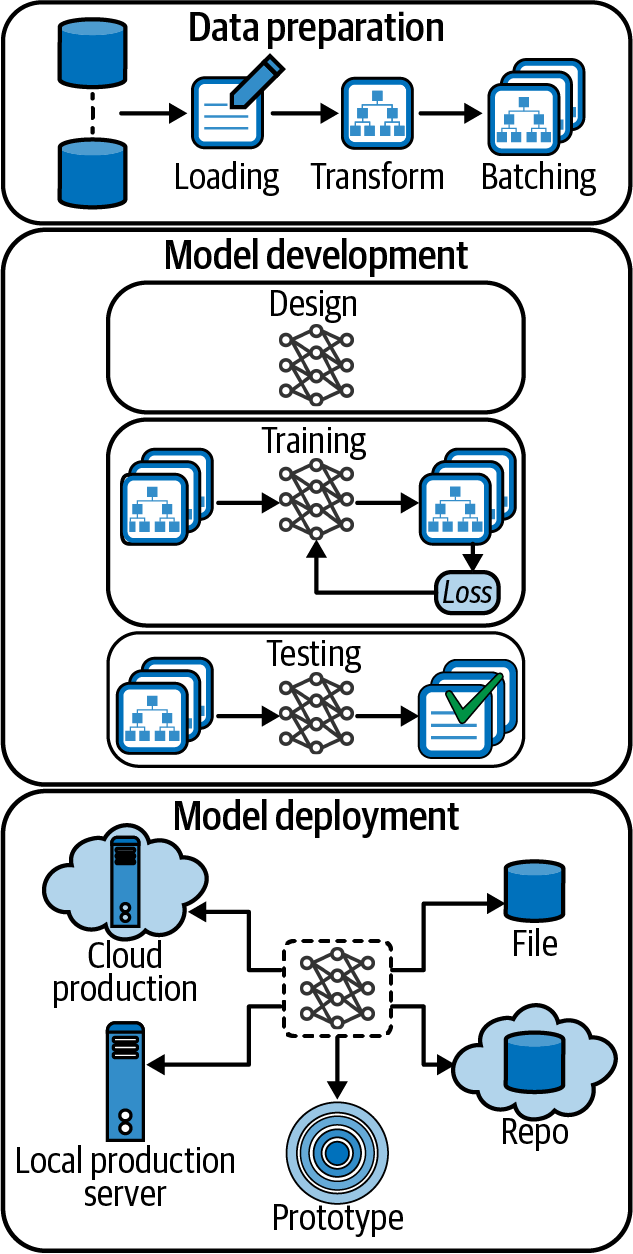
\includegraphics[width=.65\textwidth]{img/fig3-1.png}
    \caption{The basic deep learning development process}
    \label{fig3-1}
\end{figure}
\section{Data Preparation}
\subsection{Data Loading}
PyTorch provides powerful built-in classes and utilities, such as
the \textsf{Dataset}, \textsf{DataLoader}, and \textsf{Sampler} classes, for loading various types of data. The Dataset class defines how to access and
preprocess data from a file or data sources. The Sampler class
defines how to sample data from a dataset in order to create
batches, while the DataLoader class combines a dataset with a
sampler and allows you to iterate over a set of batches.

PyTorch libraries such as Torchvision and Torchtext also provide classes to support specialized data like computer vision
and natural language data. The torchvision.datasets module
is a good example of how to utilize built-in classes to load data.
The torchvision.datasets module provides a number of subclasses to load image data from popular academic datasets.

\subsection{Data Transforms}
The data might need to be adjusted
before it is passed into the NN model for training and testing. These adjustments are accomplished by applying transforms. \textbf{The beauty of using transforms in PyTorch is that you can define a sequence of transforms and apply it when the data is accessed.}

\important{The transforms are passed to the dataset class during instantiation and become part of the dataset object. The transforms are applied whenever the dataset object is accessed, returning a new result consisting of the transformed data.}

\subsection{Data Batching}
When you train your model, you will want to pass in small batches of data at each iteration. Sending data in batches not only allows more efficient training but also takes advantage of the parallel nature of
GPUs to accelerate training.

Batch processing can easily be implemented using the \textsf{torch.utils.data.DataLoader} class.

The dataloader object combines a dataset and a sampler, and
provides an iterable over the given dataset. In other words,
your training loop can use this object to sample your dataset
and apply transforms one batch at a time instead of applying
them for the complete dataset at once. This considerably
improves efficiency and speed when training and testing
models.

We need to use iter() to cast the trainloader to an iterator
and then use next() to iterate over the data one more time.
This is only necessary when accessing one batch. As we’ll see
later, our training loops will access the dataloader directly
without the need for iter() and next().

\subsection{General Data Preparation (torch.utils.data)}
You can use PyTorch to prepare other types of data as well. PyTorch libraries such as Torchtext and Torchaudio provide dataset and dataloader
classes for text and audio data, and new external libraries are
being developed all the time.

PyTorch also provides a submodule called torch.utils.data
that you can use to create your own dataset and dataloader
classes like the ones you saw in Torchvision. It consists of
Dataset, Sampler, and DataLoader classes.
\subsubsection{Dataset classes}
PyTorch supports map- and iterable-style dataset classes. A
map-style dataset is derived from the abstract class
torch.utils.data.Dataset. It implements the getitem() and
len() functions, and represents a map from (possibly nonintegral) indices/keys to data samples. For example, such a dataset, when accessed with dataset[idx], could read the idx-th
image and its corresponding label from a folder on the disk.
Map-style datasets are more commonly used than iterable-style
datasets, and all datasets that represent a map made from keys
or data samples should use this subclass.

\begin{tcolorbox}[title=TIP]
    The simplest way to create your own dataset class is to subclass the map-style torch.utils.data.Dataset class and override the \textsf{getitem()} and \textsf{len()} functions with your own code.
\end{tcolorbox}

\important{All subclasses should overwrite getitem(), which fetches a data
    sample for a given key.} Subclasses can also optionally overwrite
len(), which returns the size of the dataset by many Sampler
implementations and the default options of DataLoader.

An iterable-style dataset, on the other hand, is derived from the
torch.utils.data.IterableDataset abstract class. It implements the iter() protocol and represents an iterable over data
samples. This type of dataset is typically used when reading
data from a database or a remote server, as well as data generated in real time. Iterable datasets are useful when random
reads are expensive or uncertain, and when the batch size
depends on fetched data.

PyTorch’s torch.utils.data submodule also provides dataset
operations to convert, combine, or split dataset objects. These
operations include the following:
\begin{itemize}
    \item \textsf{TensorDataset(tensors)}: Creates a dataset object from a tensor
    \item \textsf{ConcatDataset(datasets)}: Creates a dataset from multiple datasets
    \item \textsf{ChainDataset(datasets)}: Chains multiple IterableDatasets
    \item \textsf{Subset(dataset, indices)}: Creates a subset of a dataset from specified indices
\end{itemize}
\subsubsection{Sampler classes}
In addition to dataset classes PyTorch also provides sampler
classes, which offer a way to iterate over indices of dataset samples. Sampler are derived from the torch.utils.data.Sampler base class.

Every Sampler subclass needs to implement an iter() method
to provide a way to iterate over indices of dataset elements and
a len() method that returns the length of the returned iterators. \autoref{tbl3-1} provides a list of available samplers for your reference.

\begin{table}
    \centering
    \caption{Dataset samplers (torch.utils.data)}
    \label{tbl3-1}
    \begin{tabularx}{\textwidth}{XX}
        \hline
        Sampler                                                                                      & Description                                        \\
        \hline
        SequentialSampler(data\_source)                                                              & Samples data in sequence                           \\
        RandomSampler(data\_source, replacement=False, num\_samples=None, generator=None)            & Samples data randomly                              \\
        SubsetRandomSampler(indices, generator=None)                                                 & Samples data randomly from a subset of the dataset \\
        WeightedRandomSampler(weights, num\_samples, replacement=True, generator=None)               & Samples randomly from a weighted distribution      \\
        BatchSampler(sampler, batch\_size, drop\_last)                                               & Returns a batch of samples                         \\
        distributed.DistributedSampler(dataset, num\_replicas=None, rank=None, shuffle=True, seed=0) & Samples across distributed datasets                \\
        \hline
    \end{tabularx}
\end{table}

Samplers are usually not used directly. They are often passed to
dataloaders to define the way the dataloader samples the
dataset.

\subsubsection{DataLoader classes}
The Dataset class returns a dataset object that includes data
and information about the data. The Sampler class returns the
actual data itself in a specified or random fashion. The Data
Loader class combines a dataset with a sampler and returns an
iterable.

The dataset and sampler objects are not iterables, meaning you
cannot run a for loop on them. The dataloader object solves
this problem.
\section{Model Development}
